% Replicação passo a passo da seção 4 de BC (2026). Compilar com XeLaTeX (duas passadas).
% Números e tabelas vêm de ../R/05_documento.R (pasta gerado/); nada é digitado à mão.
\documentclass[11pt,a4paper]{article}
\usepackage{fontspec}
\usepackage[brazil]{babel}
\usepackage[margin=2.3cm]{geometry}
\usepackage{amsmath,amssymb}
\usepackage{booktabs,float,graphicx,caption}
\usepackage{xcolor}
\usepackage{listings}
\usepackage[hidelinks]{hyperref}
\captionsetup{font=small,labelfont=bf}
\setlength{\parskip}{0.45em}
\setlength{\parindent}{0pt}
\lstset{basicstyle=\ttfamily\small,columns=fullflexible,frame=single,framerule=0.3pt,
  backgroundcolor=\color{gray!6},breaklines=true,upquote=true,literate={ç}{{\c{c}}}1 {ã}{{\~a}}1}
\newcommand{\Nreunioes}{115}
\newcommand{\Nsurpresas}{20}
\newcommand{\Nmeses}{172}
\newcommand{\Nmesessurp}{20}
\newcommand{\ExReuniao}{R2/2021}
\newcommand{\ExData}{17/03/2021}
\newcommand{\ExFocusData}{16/03/2021}
\newcommand{\ExAnterior}{2{,}00}
\newcommand{\ExMediana}{2{,}50}
\newcommand{\ExDecisao}{2{,}75}
\newcommand{\ExSurpresa}{0{,}25}
\newcommand{\MediaLivre}{314{,}6}
\newcommand{\MediaDir}{41{,}3}
\newcommand{\MediaTotal}{355{,}9}
\newcommand{\ParticDir}{11{,}6}
\newcommand{\PiFSTL}{6{,}514}
\newcommand{\PiRFTL}{9{,}498}
\newcommand{\BetaTL}{1{,}458}
\newcommand{\WaldTL}{1{,}458}
\newcommand{\SEivTL}{0{,}402}
\newcommand{\SEssTL}{0{,}521}
\newcommand{\FefTL}{15{,}7}
\newcommand{\BetaTLols}{1{,}324}
\newcommand{\SEolsTL}{0{,}173}
\newcommand{\NTL}{151}
\newcommand{\IniTL}{06/2011}
\newcommand{\IClTL}{0{,}67}
\newcommand{\IChTL}{2{,}25}
\newcommand{\ZZTL}{1{,}413}
\newcommand{\ZXTL}{9{,}205}
\newcommand{\ZYTL}{13{,}421}
\newcommand{\PmanTL}{6{,}514}
\newcommand{\RmanTL}{9{,}498}
\newcommand{\BmanTL}{1{,}458}
\newcommand{\SmanTL}{13{,}709}
\newcommand{\SEmanTL}{0{,}402}
\newcommand{\SEhcTL}{0{,}397}
\newcommand{\SEhomTL}{0{,}294}
\newcommand{\SSRokTL}{750{,}13}
\newcommand{\SSRssTL}{1976{,}76}
\newcommand{\KwTL}{5}
\newcommand{\LnwTL}{19}
\newcommand{\PiFSCD}{6{,}568}
\newcommand{\PiRFCD}{\ensuremath{-}17{,}714}
\newcommand{\BetaCD}{\ensuremath{-}2{,}697}
\newcommand{\WaldCD}{\ensuremath{-}2{,}697}
\newcommand{\SEivCD}{3{,}846}
\newcommand{\SEssCD}{4{,}006}
\newcommand{\FefCD}{26{,}8}
\newcommand{\BetaCDols}{\ensuremath{-}2{,}243}
\newcommand{\SEolsCD}{2{,}209}
\newcommand{\NCD}{139}
\newcommand{\IniCD}{06/2012}
\newcommand{\IClCD}{\ensuremath{-}10{,}23}
\newcommand{\IChCD}{4{,}84}
\newcommand{\ZZCD}{1{,}007}
\newcommand{\ZXCD}{6{,}617}
\newcommand{\ZYCD}{\ensuremath{-}17{,}846}
\newcommand{\PmanCD}{6{,}568}
\newcommand{\RmanCD}{\ensuremath{-}17{,}714}
\newcommand{\BmanCD}{\ensuremath{-}2{,}697}
\newcommand{\SmanCD}{647{,}520}
\newcommand{\SEmanCD}{3{,}846}
\newcommand{\SEhcCD}{4{,}255}
\newcommand{\SEhomCD}{3{,}884}
\newcommand{\SSRokCD}{82620{,}58}
\newcommand{\SSRssCD}{84774{,}64}
\newcommand{\KwCD}{12}
\newcommand{\LnwCD}{19}
\newcommand{\TotalRS}{0{,}21}
\newcommand{\TotalRSlo}{\ensuremath{-}7{,}8}
\newcommand{\TotalRShi}{8{,}2}

\newcommand{\BC}{BC (2026)}

\title{Transmissão da Selic pelo crédito:\\ a seção 4 do estudo do BC refeita passo a passo}
\author{Tiago Müller de Brito}
\date{Novembro de 2026}

\begin{document}
\maketitle

\begin{abstract}
Este documento refaz, com dados públicos, a seção 4 de \BC, \emph{Transmissão da Política Monetária
por meio do Crédito: evidência teórica e empírica}. Mostra como se monta cada variável, escreve as
duas regressões do estimador de mínimos quadrados em dois estágios com todos os coeficientes, prova
que o efeito estimado é a razão entre a forma reduzida e o primeiro estágio, e explica os erros-padrão.
Depois compara os resultados com os do BC e roda os diagnósticos que o estudo não reporta. As
páginas citadas são as impressas no relatório do BC.
\end{abstract}

\tableofcontents

%======================================================================================
\section{A pergunta e o problema}

O BC quer saber quanto uma Selic mais alta muda (i) as taxas de juros dos empréstimos e (ii) o volume
de concessões, por tipo de crédito, ao longo de 18 meses (p.~41–53).

A regressão ingênua seria a da taxa do empréstimo na Selic. Ela mistura duas coisas. A Selic afeta o
crédito, mas o Copom também escolhe a Selic olhando para o que move o crédito: quando a economia
aquece, o Copom sobe os juros e, ao mesmo tempo, a demanda por crédito cresce. O coeficiente de
mínimos quadrados ordinários (MQO) mede a soma dos dois movimentos. Em linguagem de regressão, a
Selic é \textbf{endógena}: está correlacionada com o termo de erro.

A saída do BC tem duas camadas, que vale manter separadas:
\begin{enumerate}
  \item \textbf{Estimador}: projeções locais com multiplicador cumulativo (Jordà e Taylor, 2025), que
        dizem \emph{como} medir a resposta ao longo do tempo (seção~\ref{sec:lp}).
  \item \textbf{Identificação}: uma variável instrumental, a surpresa do mercado na decisão do Copom,
        que diz \emph{qual} variação da Selic se pode tratar como exógena (seções~\ref{sec:surpresa}
        e~\ref{sec:duas}).
\end{enumerate}

%======================================================================================
\section{Os dados}\label{sec:dados}

Todas as séries vêm do Sistema Gerenciador de Séries Temporais (SGS) do BC, mensais, de março de
2011 a junho de 2025, como no estudo (p.~46).

\begin{table}[H]\centering\small
\caption{Séries usadas}
\begin{tabular}{p{5.4cm}p{4.2cm}p{5.3cm}}
\toprule
Variável & Códigos SGS & Transformação \\
\midrule
Concessões (total; PF e PJ; livres e direcionados) & 24439 a 24447 & dessazonalizadas pelo BC; $\div$ IPCA; $100\times\log$ \\
Concessões brutas (para pesos) & 20631, 20634, 20635, 20662, 20685, 20686, 20698 & R\$ milhões \\
Taxas médias de juros (mesmos recortes) & 20714, 20717, 20718, 20740, 20756, 20757, 20768 & \% a.a., em nível \\
Selic & 4189 & \% a.a., média do mês \\
IPCA & 433 & índice, $100\times\log$ \\
IBC-Br dessazonalizado & 24364 & $100\times\log$ \\
Desocupação (PNAD Contínua) & 24369 & \%, desde mar/2012 \\
\bottomrule
\end{tabular}
\end{table}

\textbf{Conferência com o BC.} A média mensal das concessões brutas na amostra é R\$~\MediaLivre{}
bilhões no crédito livre, R\$~\MediaDir{} bilhões no direcionado e R\$~\MediaTotal{} bilhões no total.
A Tabela 4.1 do BC (p.~47) traz 312,1; 41,0 e 353,2. São os mesmos dados, com pequenas revisões. O
direcionado é \ParticDir\% das concessões mensais.

\textbf{Por que log vezes 100.} Para variações pequenas, $100\times(\log a - \log b)\approx$ variação
percentual. Assim o coeficiente das concessões se lê direto em \%.

%======================================================================================
\section{O instrumento: a surpresa do Copom}\label{sec:surpresa}

\subsection{A versão do BC: DI futuro}
O BC mede a surpresa no mercado de DI futuro (p.~43–44). No dia $t$ da decisão, calcula a taxa a
termo $f_t(t+1,T)$ que o mercado embutia para o período do dia seguinte até o vencimento $T$ do
contrato, tirando da taxa do contrato o dia $t$, cuja DI já é conhecida:
\begin{equation}
(1+r_t(T))^{\,du_T/252} = (1+DI_t)^{1/252}\,\bigl(1+f_t(t+1,T)\bigr)^{(du_T-1)/252}.
\end{equation}
No fechamento do dia seguinte, a taxa do mesmo contrato é $r_{t+1}(T)$. A surpresa é
\begin{equation}
z_t = r_{t+1}(T) - f_t(t+1,T),
\end{equation}
com $10 < du_T < 40$ dias úteis (só uma reunião do Copom dentro do prazo) e $z_t=0$ quando
$|z_t|<5$ pontos-base. Como o Copom anuncia com o mercado fechado, a janela vai de um fechamento ao
outro (p.~42 e 44).

\subsection{A versão desta réplica: Focus}
O BC informa que os resultados se mantêm quando a surpresa é medida contra a pesquisa Focus
(nota~41, p.~46). É essa a versão usada aqui, porque os dados são públicos:
\begin{equation}
z_m = \underbrace{i^{\text{decidida}}_m}_{\text{meta Selic}} - \underbrace{\text{mediana}^{\text{Focus}}_m}_{\text{última pesquisa antes da reunião}},
\end{equation}
descartando a reunião se a última pesquisa tem mais de 10 dias. No mês, $z_t$ é a soma das
surpresas das reuniões do mês (zero nos meses sem reunião).

\textbf{Exemplo.} Na reunião \ExReuniao{} (\ExData), a Selic estava em \ExAnterior\%. Na pesquisa
Focus de \ExFocusData, a mediana dos analistas para essa reunião era \ExMediana\%. O Copom decidiu
\ExDecisao\%. A surpresa é $\ExDecisao - \ExMediana = \ExSurpresa$ p.p.: o mercado esperava alta, e a
alta veio maior.

\textbf{Quantas surpresas existem.} Das \Nreunioes{} reuniões da amostra, \Nsurpresas{} têm surpresa
diferente de zero; nos \Nmeses{} meses, \Nmesessurp{} têm $z_t\neq 0$. Todo o efeito é identificado
por esses eventos.

\begin{table}[H]\centering\small
\caption{Reuniões com surpresa diferente de zero (mar/2011--jun/2025)}
\begin{tabular}{llrrrr}
\toprule
Reunião & Data & Selic anterior & Mediana Focus & Decisão & Surpresa (p.p.) \\
\midrule
R3/2011 & 20/04/2011 & 11{,}75 & 12{,}25 & 12{,}00 & \ensuremath{-}0{,}25 \\
R6/2011 & 31/08/2011 & 12{,}50 & 12{,}50 & 12{,}00 & \ensuremath{-}0{,}50 \\
R2/2012 & 07/03/2012 & 10{,}50 & 10{,}00 & 9{,}75 & \ensuremath{-}0{,}25 \\
R7/2012 & 10/10/2012 & 7{,}50 & 7{,}50 & 7{,}25 & \ensuremath{-}0{,}25 \\
R3/2013 & 17/04/2013 & 7{,}25 & 7{,}25 & 7{,}50 & 0{,}25 \\
R4/2013 & 29/05/2013 & 7{,}50 & 7{,}75 & 8{,}00 & 0{,}25 \\
R1/2014 & 15/01/2014 & 10{,}00 & 10{,}25 & 10{,}50 & 0{,}25 \\
R7/2014 & 29/10/2014 & 11{,}00 & 11{,}00 & 11{,}25 & 0{,}25 \\
R8/2014 & 03/12/2014 & 11{,}25 & 11{,}50 & 11{,}75 & 0{,}25 \\
R1/2016 & 20/01/2016 & 14{,}25 & 14{,}75 & 14{,}25 & \ensuremath{-}0{,}50 \\
R1/2017 & 11/01/2017 & 13{,}75 & 13{,}25 & 13{,}00 & \ensuremath{-}0{,}25 \\
R3/2018 & 16/05/2018 & 6{,}50 & 6{,}25 & 6{,}50 & 0{,}25 \\
R5/2019 & 31/07/2019 & 6{,}50 & 6{,}25 & 6{,}00 & \ensuremath{-}0{,}25 \\
R2/2020 & 18/03/2020 & 4{,}25 & 4{,}00 & 3{,}75 & \ensuremath{-}0{,}25 \\
R3/2020 & 06/05/2020 & 3{,}75 & 3{,}25 & 3{,}00 & \ensuremath{-}0{,}25 \\
R2/2021 & 17/03/2021 & 2{,}00 & 2{,}50 & 2{,}75 & 0{,}25 \\
R7/2021 & 27/10/2021 & 6{,}25 & 7{,}50 & 7{,}75 & 0{,}25 \\
R5/2023 & 02/08/2023 & 13{,}75 & 13{,}50 & 13{,}25 & \ensuremath{-}0{,}25 \\
R8/2024 & 11/12/2024 & 11{,}25 & 12{,}00 & 12{,}25 & 0{,}25 \\
R4/2025 & 18/06/2025 & 14{,}75 & 14{,}75 & 15{,}00 & 0{,}25 \\
\bottomrule
\end{tabular}

\end{table}

\begin{figure}[H]\centering
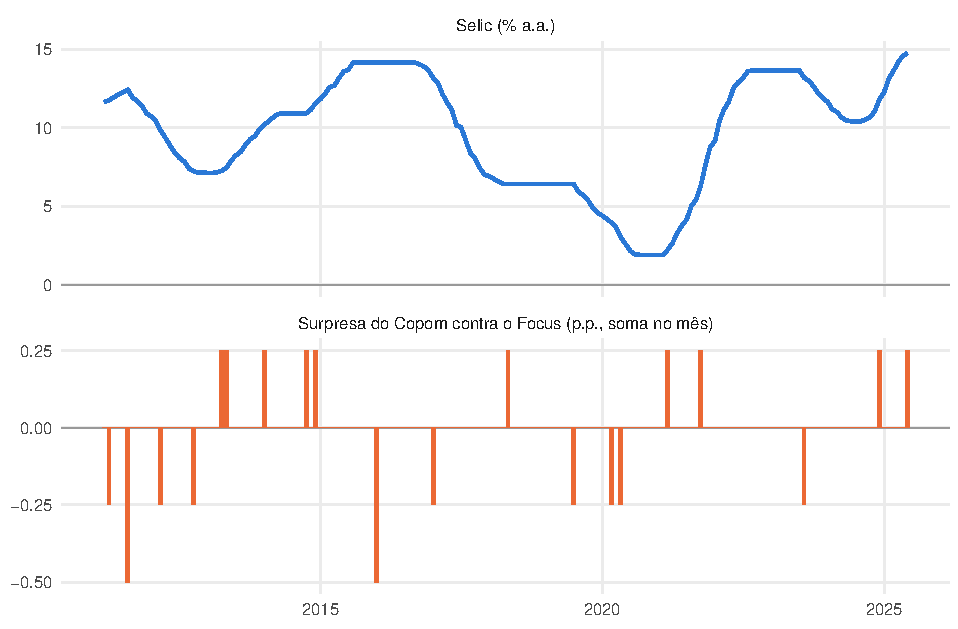
\includegraphics[width=0.92\textwidth]{gerado/fig_surpresas.pdf}
\caption{Selic e surpresas do Copom. A variação da Selic que identifica o efeito é só a dos meses com barra.}
\end{figure}

%======================================================================================
\section{A projeção local e o multiplicador cumulativo}\label{sec:lp}

Uma projeção local estima uma regressão separada para cada horizonte $h$, em vez de um sistema
inteiro (Jordà, 2005). O BC usa a versão de Jordà e Taylor (2025), que não pergunta ``quanto a
variável muda $h$ meses depois do choque'', e sim ``quanto ela muda em média, por ponto de Selic também
em média''. O motivo é que, depois de uma surpresa, o Copom continua mexendo na Selic; o multiplicador
divide uma resposta pela outra (p.~45).

Para cada mês $t$ e horizonte $h$, monte duas variáveis:
\begin{align}
Y^h_t &= \frac{1}{h+1}\sum_{j=0}^{h} y_{t+j} \;-\; y_{t-1}, \label{eq:Y}\\
X^h_t &= \frac{1}{h+1}\sum_{j=0}^{h} i_{t+j} \;-\; i_{t-1}, \label{eq:X}
\end{align}
em que $y$ é a taxa do empréstimo (ou o log das concessões) e $i$ é a Selic. A equação de interesse é
\begin{equation}\label{eq:estrutural}
Y^h_t = \beta_h\, X^h_t + W_t'\gamma_h + u^h_t ,
\end{equation}
e $\beta_h$ é o \textbf{multiplicador cumulativo}: se a Selic fica 1~p.p. mais alta, em média, entre
$t$ e $t+h$, a taxa do empréstimo fica $\beta_h$~p.p. mais alta, em média, no mesmo período. Nas
concessões, fica $\beta_h$\% maior (ou menor).

$W_t$ são os controles, todos medidos antes de $t$ (p.~46):
\begin{itemize}
  \item taxas: constante, $\Delta y_{t-1}$, $\Delta y_{t-2}$, $\Delta i_{t-1}$, $\Delta i_{t-2}$;
  \item concessões: os mesmos, mais duas defasagens da variação da desocupação ($\Delta u$), do log
        do IPCA ($\Delta p$) e do log do IBC-Br ($\Delta a$), e uma dummy de pandemia (mar/2020 a
        dez/2022).
\end{itemize}
O BC escolhe as defasagens pelo critério BIC e inclui também o índice de incerteza IIE-Br; aqui são
duas defasagens fixas e sem o IIE-Br, que o BC diz não mudar o resultado (nota~41).

\textbf{Exemplo de montagem}, taxa do crédito livre com $h=18$, em volta da reunião \ExReuniao.
Cada linha é um mês $t$; $\bar{i}_{t,t+18}$ é a média da Selic de $t$ a $t+18$.

\begin{table}[H]\centering\small
\caption{Construção de $X^{18}_t$ e $Y^{18}_t$ (taxa do crédito livre, \% a.a.)}
\begin{tabular}{lrrrrrrr}
\toprule
Mês $t$ & $z_t$ & $i_{t-1}$ & $\bar{i}_{t,t+18}$ & $X^{18}_t$ & $y_{t-1}$ & $\bar{y}_{t,t+18}$ & $Y^{18}_t$ \\
\midrule
02/2021 & 0{,}00 & 1{,}90 & 7{,}67 & 5{,}77 & 27{,}91 & 32{,}99 & 5{,}08 \\
03/2021 & 0{,}25 & 1{,}90 & 8{,}29 & 6{,}39 & 27{,}67 & 33{,}63 & 5{,}96 \\
04/2021 & 0{,}00 & 2{,}23 & 8{,}89 & 6{,}66 & 27{,}95 & 34{,}35 & 6{,}40 \\
05/2021 & 0{,}00 & 2{,}65 & 9{,}47 & 6{,}82 & 28{,}66 & 35{,}07 & 6{,}41 \\
06/2021 & 0{,}00 & 3{,}29 & 10{,}01 & 6{,}72 & 27{,}99 & 35{,}76 & 7{,}77 \\
\bottomrule
\end{tabular}

\end{table}

Leia a linha de março de 2021: $X^{18}_t$ é quanto a Selic média dos 19 meses seguintes ficou acima
da Selic de fevereiro; $Y^{18}_t$ é o mesmo para a taxa do crédito livre. A regressão compara esses
dois números entre os meses, usando só a parte de $X^{18}_t$ que a surpresa explica.

O último mês $t$ que entra na regressão é dezembro de 2023: a média de $t$ a $t+18$ precisa de dados
até junho de 2025, o fim da amostra. Por isso as tabelas a seguir terminam em 12/2023.

%======================================================================================
% Seção 5 de replicacao_secao4.tex: as duas regressões do MQ2E, passo a passo.
% Números de gerado/numeros.tex (R/05_documento.R).
\section{As duas regressões, passo a passo}\label{sec:duas}

\subsection{Por que MQO não serve}
Em~\eqref{eq:estrutural}, $X^h_t$ contém a reação do Copom ao que ele vê da economia, e o erro
$u^h_t$ contém o que move o crédito além da Selic. Para ver o viés, residualize tudo nos controles
$W$ (Frisch--Waugh--Lovell): seja $M_W = I - W(W'W)^{-1}W'$ e $\tilde a = M_W a$ o resíduo de $a$
regredido em $W$. O MQO do coeficiente da Selic é
\begin{equation}\label{eq:mqo}
\hat\beta^{\,MQO} = \frac{\tilde X'\tilde Y}{\tilde X'\tilde X}
                  = \beta + \frac{\tilde X'u}{\tilde X'\tilde X}.
\end{equation}
Se o Copom reage ao que está em $u$, então $\tilde X'u \neq 0$ mesmo em amostras grandes, e o MQO
erra por esse termo. A variável instrumental troca, no numerador e no denominador, o $\tilde X$ por
uma variável que não reage a $u$.

\subsection{As condições da variável instrumental}
Um instrumento $z_t$ precisa de duas condições, dados os controles $W_t$:
\begin{enumerate}
  \item \textbf{Relevância}: $z_t$ move $X^h_t$, isto é, $\tilde z'\tilde X \neq 0$. Testável, pelo primeiro estágio.
  \item \textbf{Exogeneidade e exclusão}: $\operatorname{E}[z_t\,u^h_t\mid W_t]=0$; $z_t$ só afeta
        $Y^h_t$ por meio de $X^h_t$. \textbf{Não testável} com um instrumento e uma variável endógena:
        ``the exclusion or exogeneity condition cannot be tested'' e ``the reliability of an instrument
        relies on argumentation, not on empirical testing'' (Verbeek, 2017, p.~154).
\end{enumerate}
O BC escreve as duas como hipótese (p.~45--46) e as defende numa frase: as surpresas ``são
plausivelmente ortogonais às condições do mercado de crédito'' (p.~45). A ameaça principal é o efeito
informação (p.~42--43; Nakamura e Steinsson, 2018, p.~76).

\subsection{As três regressões}
O MQ2E costuma ser apresentado como duas regressões; vale escrever também a terceira, que liga as
duas. Os controles $W_t$ entram nas três.
\begin{align}
\text{Primeiro estágio:}\quad & X^h_t = \pi_h\, z_t + W_t'\delta_h + v^h_t, \label{eq:fs}\\
\text{Forma reduzida:}\quad & Y^h_t = \rho_h\, z_t + W_t'\lambda_h + e^h_t, \label{eq:rf}\\
\text{Segundo estágio:}\quad & Y^h_t = \beta_h\, \widehat{X}^h_t + W_t'\gamma_h + \text{erro},
\quad \widehat{X}^h_t = \hat\pi_h z_t + W_t'\hat\delta_h. \label{eq:ss}
\end{align}
O primeiro estágio mede quanto a surpresa move a Selic; a forma reduzida, quanto a surpresa move o
crédito; o segundo estágio usa só a parte da Selic que a surpresa (e os controles) explicam.

\subsection{O estimador em uma linha}
Com um instrumento e uma variável endógena, depois de residualizar nos controles:
\begin{align}
\text{1º estágio:}\quad & \hat\pi = \frac{\tilde z'\tilde X}{\tilde z'\tilde z}, \label{eq:pi}\\
\text{forma reduzida:}\quad & \hat\rho = \frac{\tilde z'\tilde Y}{\tilde z'\tilde z}, \label{eq:rho}\\
\text{MQ2E:}\quad & \hat\beta = \frac{\tilde z'\tilde Y}{\tilde z'\tilde X} = \frac{\hat\rho}{\hat\pi}. \label{eq:b2sls}
\end{align}
Compare com~\eqref{eq:mqo}: o MQ2E é o MQO com $\tilde z$ no lugar de $\tilde X$ nos dois
produtos. Substituindo $\tilde Y = \beta\tilde X + \tilde u$,
\begin{equation}\label{eq:erro_vi}
\hat\beta - \beta = \frac{\tilde z'u}{\tilde z'\tilde X},
\end{equation}
que vai a zero se $z$ não anda junto com $u$ (exogeneidade) e se o denominador não é perto de zero
(relevância). Se $\tilde z'\tilde X\approx0$, qualquer correlação pequena entre $z$ e $u$ explode:
é o problema do instrumento fraco.

\textbf{Em matrizes.} Com $\bar X=[X\ \ W]$, $\bar Z=[z\ \ W]$ e
$P_{\bar Z}=\bar Z(\bar Z'\bar Z)^{-1}\bar Z'$, o MQ2E é
\[
\hat\theta=(\bar X'P_{\bar Z}\bar X)^{-1}\bar X'P_{\bar Z}\,Y,
\qquad\text{e, no caso exatamente identificado,}\qquad
\hat\theta=(\bar Z'\bar X)^{-1}\bar Z'Y.
\]
A coordenada de $X$ nesse vetor é exatamente~\eqref{eq:b2sls}. Os ``dois estágios'' são a leitura de $P_{\bar Z}\bar X$: primeiro
projeta-se $X$ no espaço de $(z,W)$, depois regride-se $Y$ na projeção.

%-------------------------------------------------------------------------------------
\subsection{Exemplo 1 com todos os números: taxa do crédito livre, $h=18$}

\paragraph{Passo 1: montar as variáveis.} $Y^{18}_t$ e $X^{18}_t$ como em~\eqref{eq:Y}
e~\eqref{eq:X}; $z_t$ é a surpresa do mês; $W_t$ tem \KwTL{} colunas: constante, $\Delta y_{t-1}$,
$\Delta y_{t-2}$, $\Delta i_{t-1}$, $\Delta i_{t-2}$. São $N=\NTL$ meses, de \IniTL{} a 12/2023.

\paragraph{Passo 2: residualizar nos controles.} Regride-se $z$, $X$ e $Y$, cada um, em $W$ e
guardam-se os resíduos. Alguns meses:
\begin{table}[H]\centering\small
\caption{Variáveis residualizadas nos controles (taxa do crédito livre)}
\begin{tabular}{lrrrr}
\toprule
Mês $t$ & $\tilde z_t$ & $\tilde X_t$ & $\tilde Y_t$ & $g_t=\tilde z_t\hat u_t$ \\
\midrule
01/2021 & 0{,}010 & 4{,}907 & 6{,}927 & \ensuremath{-}0{,}002 \\
02/2021 & \ensuremath{-}0{,}003 & 5{,}848 & 4{,}831 & 0{,}012 \\
03/2021 & 0{,}242 & 7{,}507 & 6{,}803 & \ensuremath{-}1{,}001 \\
04/2021 & \ensuremath{-}0{,}003 & 5{,}240 & 3{,}808 & 0{,}010 \\
05/2021 & \ensuremath{-}0{,}005 & 4{,}927 & 2{,}328 & 0{,}026 \\
06/2021 & \ensuremath{-}0{,}006 & 3{,}816 & 1{,}890 & 0{,}022 \\
\bottomrule
\end{tabular}

\end{table}
Somando os produtos em todos os \NTL{} meses:
\[
\tilde z'\tilde z = \ZZTL,\qquad \tilde z'\tilde X = \ZXTL,\qquad \tilde z'\tilde Y = \ZYTL.
\]

\paragraph{Passo 3: primeiro estágio.} Por~\eqref{eq:pi}, $\hat\pi=\ZXTL/\ZZTL=\PmanTL$: uma surpresa
de 1~p.p. vem acompanhada de uma Selic média, nos 19 meses seguintes, $\PmanTL$~p.p. acima da do
mês anterior, já descontados os controles. As surpresas da amostra são de 0,25 ou 0,50~p.p., então
uma surpresa típica corresponde a um quarto disso; o coeficiente é grande porque as surpresas
costumam cair no começo de ciclos de juros. É o coeficiente de $z_t$ na regressão completa:
\begin{table}[H]\centering\small
\caption{Primeiro estágio, equação~\eqref{eq:fs}: $X^{18}_t$ na surpresa e nos controles}
\begin{tabular}{lrrr}
\toprule
Regressor & Coeficiente & Erro-padrão NW & $t$ \\
\midrule
$z_t$ (surpresa do Copom) & 6{,}514 & 1{,}645 & 3{,}96 \\
$\Delta y_{t-1}$ & \ensuremath{-}0{,}164 & 0{,}152 & \ensuremath{-}1{,}07 \\
$\Delta y_{t-2}$ & \ensuremath{-}0{,}434 & 0{,}185 & \ensuremath{-}2{,}34 \\
$\Delta i_{t-1}$ & 3{,}932 & 0{,}734 & 5{,}36 \\
$\Delta i_{t-2}$ & 1{,}202 & 0{,}491 & 2{,}45 \\
Constante & 0{,}044 & 0{,}528 & 0{,}08 \\
\midrule
\multicolumn{4}{l}{$N$ = 151 meses (06/2011 a 12/2023); $R^2$ = 0{,}395} \\
\bottomrule
\end{tabular}

\end{table}
O F efetivo é o quadrado da estatística $t$ de $z_t$ com erro de Newey-West: $\FefTL$. Acima de 10,
a regra prática (Verbeek, 2017, p.~153).

\paragraph{Passo 4: forma reduzida.} Por~\eqref{eq:rho}, $\hat\rho=\ZYTL/\ZZTL=\RmanTL$: a mesma
surpresa vem acompanhada de uma taxa do crédito livre $\RmanTL$~p.p. mais alta, no mesmo sentido.
\begin{table}[H]\centering\small
\caption{Forma reduzida, equação~\eqref{eq:rf}: $Y^{18}_t$ na surpresa e nos controles}
\begin{tabular}{lrrr}
\toprule
Regressor & Coeficiente & Erro-padrão NW & $t$ \\
\midrule
$z_t$ (surpresa do Copom) & 9{,}498 & 3{,}394 & 2{,}80 \\
$\Delta y_{t-1}$ & \ensuremath{-}0{,}130 & 0{,}291 & \ensuremath{-}0{,}45 \\
$\Delta y_{t-2}$ & \ensuremath{-}0{,}423 & 0{,}275 & \ensuremath{-}1{,}54 \\
$\Delta i_{t-1}$ & 6{,}753 & 1{,}018 & 6{,}64 \\
$\Delta i_{t-2}$ & 3{,}437 & 0{,}825 & 4{,}17 \\
Constante & 0{,}272 & 0{,}847 & 0{,}32 \\
\midrule
\multicolumn{4}{l}{$N$ = 151 meses (06/2011 a 12/2023); $R^2$ = 0{,}493} \\
\bottomrule
\end{tabular}

\end{table}

\paragraph{Passo 5: segundo estágio.} Por~\eqref{eq:b2sls}, $\hat\beta=\ZYTL/\ZXTL=\BmanTL$, igual
a $\hat\rho/\hat\pi=\RmanTL/\PmanTL$ e igual ao coeficiente de $\widehat X$ na regressão do
segundo estágio:
\begin{table}[H]\centering\small
\caption{Segundo estágio, equação~\eqref{eq:ss}: $Y^{18}_t$ no valor previsto e nos controles}
\begin{tabular}{lrrr}
\toprule
Regressor & Coeficiente & Erro-padrão NW & $t$ \\
\midrule
$\widehat{X}^h_t$ (valor previsto no 1º estágio) & 1{,}458 & 0{,}521 & 2{,}80 \\
$\Delta y_{t-1}$ & 0{,}108 & 0{,}316 & 0{,}34 \\
$\Delta y_{t-2}$ & 0{,}209 & 0{,}282 & 0{,}74 \\
$\Delta i_{t-1}$ & 1{,}020 & 2{,}397 & 0{,}43 \\
$\Delta i_{t-2}$ & 1{,}684 & 1{,}214 & 1{,}39 \\
Constante & 0{,}207 & 0{,}844 & 0{,}25 \\
\midrule
\multicolumn{4}{l}{$N$ = 151 meses (06/2011 a 12/2023); $R^2$ = 0{,}493} \\
\bottomrule
\end{tabular}

\end{table}
Lê-se: uma Selic 1~p.p. mais alta, em média, nos 19 meses deixa a taxa média do crédito livre
$\BetaTL$~p.p. mais alta no mesmo período. O BC obtém 1,05 (p.~47). O $R^2$ do segundo estágio é
igual ao da forma reduzida porque $\widehat X$ é combinação de $z$ e $W$: as duas regressões usam o
mesmo espaço de regressores.

\paragraph{Passo 6: que variação da Selic a regressão usou.} A tabela a seguir põe lado a lado
$X_t$ (o que a Selic fez) e $\widehat X_t$ (a parte que a surpresa e os controles explicam):
\begin{table}[H]\centering\small
\caption{O que entra em cada regressão, em volta do início do ciclo de alta de 2021}
\resizebox{\textwidth}{!}{\begin{tabular}{lrrrrrrr}
\toprule
Mês $t$ & $z_t$ & $X^{18}_t$ & $\widehat{X}^{18}_t$ & $Y^{18}_t$ & $\hat\beta X_t + W_t'\hat\gamma$ & $\hat u_t$ (certo) & $\hat e_t$ (2º estágio à mão) \\
\midrule
01/2021 & 0{,}00 & 5{,}15 & 0{,}31 & 7{,}34 & 7{,}57 & \ensuremath{-}0{,}23 & 6{,}83 \\
02/2021 & 0{,}00 & 5{,}77 & \ensuremath{-}0{,}10 & 5{,}08 & 8{,}77 & \ensuremath{-}3{,}69 & 4{,}86 \\
03/2021 & 0{,}25 & 6{,}39 & 0{,}45 & 5{,}96 & 10{,}10 & \ensuremath{-}4{,}14 & 4{,}51 \\
04/2021 & 0{,}00 & 6{,}66 & 1{,}40 & 6{,}40 & 10{,}23 & \ensuremath{-}3{,}83 & 3{,}83 \\
05/2021 & 0{,}00 & 6{,}82 & 1{,}86 & 6{,}41 & 11{,}27 & \ensuremath{-}4{,}86 & 2{,}38 \\
06/2021 & 0{,}00 & 6{,}72 & 2{,}87 & 7{,}77 & 11{,}44 & \ensuremath{-}3{,}67 & 1{,}95 \\
\bottomrule
\end{tabular}
}
\end{table}
Em 2021 a Selic média dos 19 meses seguintes ficou cerca de 5 a 7~p.p. acima da do mês anterior
($X_t$), mas $\widehat X_t$ fica perto de zero até março: o mercado já esperava quase todo o ciclo.
Depois de março, $\widehat X_t$ sobe porque as altas já feitas entram nos controles
($\Delta i_{t-1}$, $\Delta i_{t-2}$), não por novas surpresas. A VI ignora a parte antecipada e
estima $\beta$ só com a variação ligada à surpresa. É isso que a protege da reação do
Copom à economia, e é também por isso que ela tem pouca informação (\Nmesessurp{} meses com
$z_t\neq0$ na amostra).

\paragraph{Passo 7: os resíduos certos.} O resíduo do modelo usa a Selic de verdade:
$\hat u_t = Y_t - \hat\beta X_t - W_t'\hat\gamma$. Quem roda o segundo estágio à mão obtém
$\hat e_t = Y_t - \hat\beta \widehat X_t - W_t'\hat\gamma$, com os mesmos coeficientes e o resíduo
errado (as duas últimas colunas da tabela acima). A soma dos quadrados dos resíduos certos é
$\SSRokTL$; a dos errados, $\SSRssTL$. O erro-padrão que sai do segundo estágio à mão ($\SEssTL$) é,
por isso, diferente do correto ($\SEivTL$).

\paragraph{Passo 8: o erro-padrão de Newey-West, à mão.} De~\eqref{eq:erro_vi},
$\hat\beta-\beta = \sum_t g_t / \tilde z'\tilde X$ com $g_t=\tilde z_t u_t$ (última coluna da
tabela do passo 2, com $\hat u_t$ no lugar de $u_t$). Então
\begin{equation}\label{eq:nw}
\widehat{\operatorname{Var}}(\hat\beta) = \frac{\hat S}{(\tilde z'\tilde X)^2},\qquad
\hat S = \sum_t g_t^2 + 2\sum_{j=1}^{L}\Bigl(1-\frac{j}{L+1}\Bigr)\sum_t g_t\,g_{t-j}.
\end{equation}
O primeiro termo de $\hat S$ trata a heterocedasticidade; o segundo, a correlação entre meses
próximos, com pesos que caem linearmente (Bartlett). Usa-se $L=h+1=\LnwTL$ porque $Y^{18}_t$ e
$Y^{18}_{t+1}$ compartilham 18 dos 19 meses: os erros de meses vizinhos são correlacionados por
construção. No exemplo, $\hat S=\SmanTL$ e
\[
\widehat{\text{ep}}(\hat\beta)=\frac{\sqrt{\hat S}}{|\tilde z'\tilde X|}=\frac{\sqrt{\SmanTL}}{\ZXTL}=\SEmanTL,
\]
o mesmo valor do pacote (\texttt{sandwich::NeweyWest}). Para comparar: sem o termo de
autocorrelação, o erro-padrão seria $\SEhcTL$; supondo erros homocedásticos e independentes,
$\SEhomTL$. O intervalo de 95\% é $\hat\beta\pm1{,}96\,\widehat{\text{ep}} = [\IClTL;\ \IChTL]$.

%-------------------------------------------------------------------------------------
\subsection{Exemplo 2: concessões a empresas com recursos direcionados, $h=18$}
Mesmos passos; agora $W_t$ tem \KwCD{} colunas (as das taxas mais duas defasagens da variação da
desocupação, do log do IPCA e do log do IBC-Br, e a dummy de pandemia), e a amostra começa em
\IniCD{} porque a desocupação da PNAD Contínua só existe desde 2012 ($N=\NCD$).

\begin{table}[H]\centering\small
\caption{Primeiro estágio: $X^{18}_t$ na surpresa (amostra das concessões)}
\begin{tabular}{lrrr}
\toprule
Regressor & Coeficiente & Erro-padrão NW & $t$ \\
\midrule
$z_t$ (surpresa do Copom) & 6{,}568 & 1{,}269 & 5{,}18 \\
Dummy de pandemia & 2{,}823 & 1{,}124 & 2{,}51 \\
$\Delta y_{t-1}$ & 0{,}009 & 0{,}007 & 1{,}23 \\
$\Delta y_{t-2}$ & 0{,}006 & 0{,}006 & 0{,}98 \\
$\Delta i_{t-1}$ & 1{,}827 & 0{,}472 & 3{,}87 \\
$\Delta i_{t-2}$ & \ensuremath{-}0{,}244 & 0{,}679 & \ensuremath{-}0{,}36 \\
$\Delta u_{t-1}$ & \ensuremath{-}0{,}221 & 0{,}575 & \ensuremath{-}0{,}38 \\
$\Delta u_{t-2}$ & \ensuremath{-}0{,}522 & 0{,}568 & \ensuremath{-}0{,}92 \\
$\Delta p_{t-1}$ & 1{,}267 & 0{,}377 & 3{,}36 \\
$\Delta p_{t-2}$ & 1{,}115 & 0{,}400 & 2{,}79 \\
$\Delta a_{t-1}$ & 0{,}029 & 0{,}081 & 0{,}36 \\
$\Delta a_{t-2}$ & \ensuremath{-}0{,}022 & 0{,}050 & \ensuremath{-}0{,}45 \\
Constante & \ensuremath{-}1{,}612 & 0{,}765 & \ensuremath{-}2{,}11 \\
\midrule
\multicolumn{4}{l}{$N$ = 139 meses (06/2012 a 12/2023); $R^2$ = 0{,}571} \\
\bottomrule
\end{tabular}

\end{table}
\begin{table}[H]\centering\small
\caption{Forma reduzida: $Y^{18}_t$ (log das concessões $\times100$) na surpresa}
\begin{tabular}{lrrr}
\toprule
Regressor & Coeficiente & Erro-padrão NW & $t$ \\
\midrule
$z_t$ (surpresa do Copom) & \ensuremath{-}17{,}714 & 26{,}312 & \ensuremath{-}0{,}67 \\
Dummy de pandemia & 9{,}912 & 9{,}499 & 1{,}04 \\
$\Delta y_{t-1}$ & \ensuremath{-}0{,}568 & 0{,}098 & \ensuremath{-}5{,}82 \\
$\Delta y_{t-2}$ & \ensuremath{-}0{,}289 & 0{,}122 & \ensuremath{-}2{,}36 \\
$\Delta i_{t-1}$ & 0{,}604 & 8{,}703 & 0{,}07 \\
$\Delta i_{t-2}$ & \ensuremath{-}1{,}647 & 8{,}492 & \ensuremath{-}0{,}19 \\
$\Delta u_{t-1}$ & \ensuremath{-}5{,}893 & 9{,}787 & \ensuremath{-}0{,}60 \\
$\Delta u_{t-2}$ & \ensuremath{-}21{,}397 & 12{,}576 & \ensuremath{-}1{,}70 \\
$\Delta p_{t-1}$ & \ensuremath{-}14{,}426 & 6{,}488 & \ensuremath{-}2{,}22 \\
$\Delta p_{t-2}$ & 0{,}253 & 5{,}827 & 0{,}04 \\
$\Delta a_{t-1}$ & \ensuremath{-}2{,}657 & 1{,}940 & \ensuremath{-}1{,}37 \\
$\Delta a_{t-2}$ & \ensuremath{-}2{,}334 & 1{,}317 & \ensuremath{-}1{,}77 \\
Constante & \ensuremath{-}0{,}033 & 7{,}836 & \ensuremath{-}0{,}00 \\
\midrule
\multicolumn{4}{l}{$N$ = 139 meses (06/2012 a 12/2023); $R^2$ = 0{,}284} \\
\bottomrule
\end{tabular}

\end{table}
\begin{table}[H]\centering\small
\caption{Segundo estágio: $Y^{18}_t$ no valor previsto}
\begin{tabular}{lrrr}
\toprule
Regressor & Coeficiente & Erro-padrão NW & $t$ \\
\midrule
$\widehat{X}^h_t$ (valor previsto no 1º estágio) & \ensuremath{-}2{,}697 & 4{,}006 & \ensuremath{-}0{,}67 \\
Dummy de pandemia & 17{,}527 & 13{,}937 & 1{,}26 \\
$\Delta y_{t-1}$ & \ensuremath{-}0{,}545 & 0{,}091 & \ensuremath{-}6{,}00 \\
$\Delta y_{t-2}$ & \ensuremath{-}0{,}272 & 0{,}115 & \ensuremath{-}2{,}36 \\
$\Delta i_{t-1}$ & 5{,}531 & 11{,}082 & 0{,}50 \\
$\Delta i_{t-2}$ & \ensuremath{-}2{,}304 & 8{,}325 & \ensuremath{-}0{,}28 \\
$\Delta u_{t-1}$ & \ensuremath{-}6{,}490 & 10{,}011 & \ensuremath{-}0{,}65 \\
$\Delta u_{t-2}$ & \ensuremath{-}22{,}805 & 12{,}206 & \ensuremath{-}1{,}87 \\
$\Delta p_{t-1}$ & \ensuremath{-}11{,}009 & 9{,}437 & \ensuremath{-}1{,}17 \\
$\Delta p_{t-2}$ & 3{,}261 & 6{,}937 & 0{,}47 \\
$\Delta a_{t-1}$ & \ensuremath{-}2{,}578 & 1{,}956 & \ensuremath{-}1{,}32 \\
$\Delta a_{t-2}$ & \ensuremath{-}2{,}394 & 1{,}318 & \ensuremath{-}1{,}82 \\
Constante & \ensuremath{-}4{,}382 & 9{,}068 & \ensuremath{-}0{,}48 \\
\midrule
\multicolumn{4}{l}{$N$ = 139 meses (06/2012 a 12/2023); $R^2$ = 0{,}284} \\
\bottomrule
\end{tabular}

\end{table}

\textbf{As contas.} $\tilde z'\tilde z=\ZZCD$, $\tilde z'\tilde X=\ZXCD$, $\tilde z'\tilde Y=\ZYCD$.
Primeiro estágio $\hat\pi=\PmanCD$; forma reduzida $\hat\rho=\RmanCD$; $\hat\beta=\ZYCD/\ZXCD=\BmanCD$:
por ponto de Selic, as concessões direcionadas a empresas ficam $\BetaCD$\% menores em média nos 18
meses. O BC reporta $-5{,}3$\%, significante (p.~51). Erro-padrão de Newey-West $\SEmanCD$ (sem
autocorrelação, $\SEhcCD$; homocedástico, $\SEhomCD$); intervalo $[\IClCD;\ \IChCD]$, com o zero
dentro. F efetivo $\FefCD$.

Note que a forma reduzida já conta a história toda: a surpresa tem coeficiente $\PiRFCD$ com
estatística $t$ pequena, isto é, não há relação detectável entre surpresas e concessões
direcionadas a empresas nesta amostra. Como $\hat\beta=\hat\rho/\hat\pi$ e o primeiro estágio é
forte, o MQ2E só reescala essa forma reduzida imprecisa em unidades de Selic.

\subsection{MQO contra VI}
Sem instrumento, o MQO de~\eqref{eq:estrutural} dá $\BetaTLols$ para a taxa do crédito livre
(contra $\BetaTL$ por VI) e $\BetaCDols$ para as concessões direcionadas a empresas (contra
$\BetaCD$). Por~\eqref{eq:mqo}, a diferença é uma estimativa do viés $\tilde X'u/\tilde X'\tilde X$,
se o instrumento for válido.


%======================================================================================
\section{Todos os resultados ($h=18$) contra os do BC}

\begin{table}[H]\centering\scriptsize
\caption{Repasse para as taxas de juros (p.p. por p.p. de Selic)}
\resizebox{\textwidth}{!}{\begin{tabular}{lrrrrrl}
\toprule
Série & Multiplicador & IC 95\% & F efetivo & Anderson-Rubin & MQO & BC (2026) \\
\midrule
Total & 1{,}00 & [0{,}57; 1{,}42] & 16{,}1 & [0{,}52; 1{,}48] & 0{,}88 & só no gráfico \\
Recursos livres & 1{,}46 & [0{,}67; 2{,}25] & 15{,}7 & [0{,}60; 2{,}41] & 1{,}32 & 1{,}05 \\
Recursos direcionados & 0{,}28 & [0{,}12; 0{,}44] & 20{,}0 & [0{,}08; 0{,}43] & 0{,}29 & 0{,}28 \\
PJ, livres & 1{,}24 & [0{,}91; 1{,}58] & 20{,}1 & [0{,}93; 1{,}67] & 1{,}13 & só no gráfico \\
PF, livres & 1{,}72 & [0{,}59; 2{,}85] & 16{,}3 & [0{,}48; 3{,}07] & 1{,}55 & só no gráfico \\
PJ, direcionados & 0{,}15 & [\ensuremath{-}0{,}15; 0{,}45] & 19{,}1 & [\ensuremath{-}0{,}24; 0{,}43] & 0{,}31 & só no gráfico \\
PF, direcionados & 0{,}36 & [0{,}25; 0{,}46] & 20{,}1 & [0{,}24; 0{,}47] & 0{,}30 & só no gráfico \\
\bottomrule
\end{tabular}
}
\end{table}

\begin{table}[H]\centering\scriptsize
\caption{Resposta das concessões (\% por p.p. de Selic)}
\resizebox{\textwidth}{!}{\begin{tabular}{lrrrrrl}
\toprule
Série & Multiplicador & IC 95\% & F efetivo & Anderson-Rubin & MQO & BC (2026) \\
\midrule
Total & 0{,}06 & [\ensuremath{-}2{,}20; 2{,}32] & 31{,}7 & [\ensuremath{-}2{,}15; 2{,}65] & \ensuremath{-}0{,}18 & só no gráfico \\
Recursos livres & 0{,}42 & [\ensuremath{-}1{,}48; 2{,}32] & 29{,}4 & [\ensuremath{-}1{,}45; 2{,}55] & 0{,}07 & só no gráfico \\
Recursos direcionados & \ensuremath{-}2{,}03 & [\ensuremath{-}6{,}52; 2{,}47] & 28{,}2 & [\ensuremath{-}6{,}50; 3{,}20] & \ensuremath{-}1{,}77 & só no gráfico \\
PJ, total & 0{,}93 & [\ensuremath{-}2{,}02; 3{,}88] & 28{,}6 & [\ensuremath{-}1{,}90; 4{,}40] & \ensuremath{-}0{,}24 & só no gráfico \\
PF, total & \ensuremath{-}0{,}34 & [\ensuremath{-}2{,}08; 1{,}39] & 25{,}5 & [\ensuremath{-}2{,}20; 1{,}50] & 0{,}04 & só no gráfico \\
PJ, livres & 1{,}13 & [\ensuremath{-}1{,}23; 3{,}48] & 30{,}9 & [\ensuremath{-}1{,}10; 3{,}90] & 0{,}01 & \ensuremath{-}0{,}3 (n.s.) \\
PF, livres & \ensuremath{-}0{,}14 & [\ensuremath{-}1{,}81; 1{,}53] & 26{,}1 & [\ensuremath{-}1{,}95; 1{,}60] & 0{,}26 & \ensuremath{-}0{,}9 (n.s.) \\
PJ, direcionados & \ensuremath{-}2{,}70 & [\ensuremath{-}10{,}23; 4{,}84] & 26{,}8 & [\ensuremath{-}10{,}05; 6{,}30] & \ensuremath{-}2{,}24 & \ensuremath{-}5{,}3 \\
PF, direcionados & \ensuremath{-}1{,}92 & [\ensuremath{-}4{,}99; 1{,}14] & 28{,}8 & [\ensuremath{-}5{,}10; 1{,}45] & \ensuremath{-}1{,}38 & \ensuremath{-}2{,}8 \\
\bottomrule
\end{tabular}
}
\end{table}

As taxas se reproduzem: o direcionado sai igual ao do BC, e o livre sai acima de 1, como lá. Nas
concessões, a direção é a do BC (direcionado cai, livre não), mas nenhuma resposta é significante a
95\%, e o total fica parado. Em reais, o efeito sobre as concessões totais é de R\$~\TotalRS{} bilhão
por mês, com intervalo de R\$~\TotalRSlo{} a \TotalRShi{} bilhões.

\begin{figure}[H]\centering
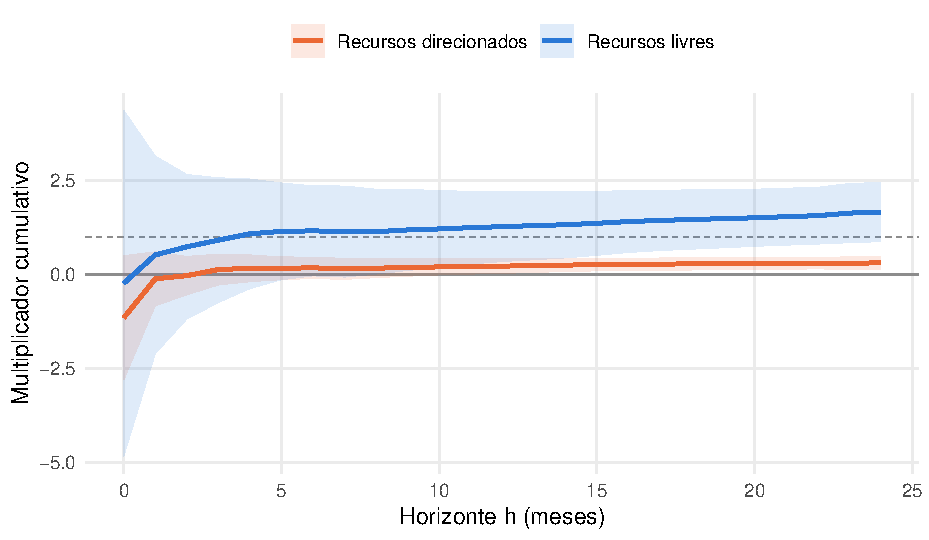
\includegraphics[width=0.85\textwidth]{gerado/fig_traj_taxas.pdf}
\caption{Multiplicador cumulativo das taxas por horizonte, com intervalo de 95\%. A linha tracejada é o repasse completo.}
\end{figure}

\begin{figure}[H]\centering
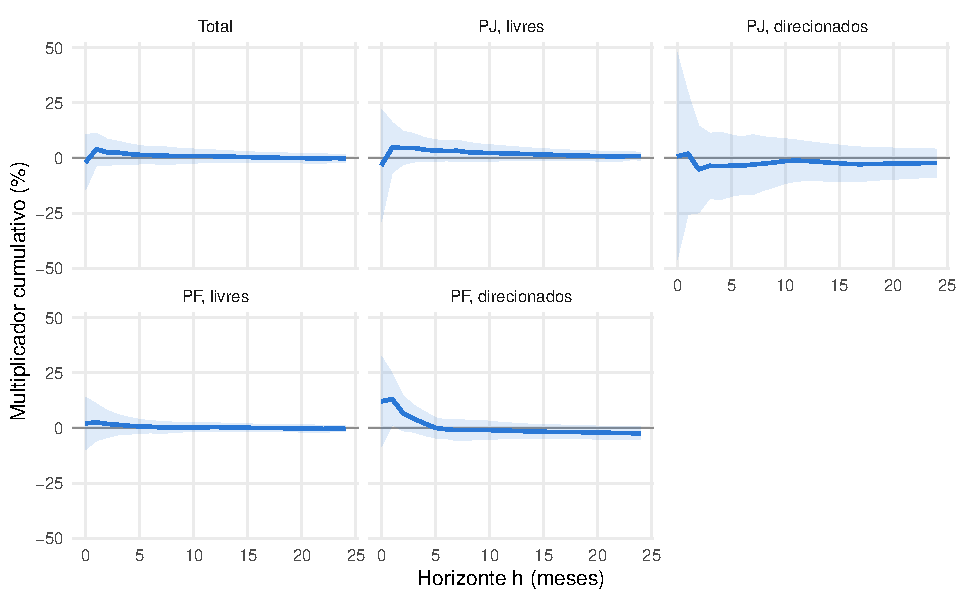
\includegraphics[width=0.95\textwidth]{gerado/fig_traj_volumes.pdf}
\caption{Multiplicador cumulativo das concessões por horizonte, com intervalo de 95\%.}
\end{figure}

%======================================================================================
\section{Diagnósticos que o estudo não reporta}

\textbf{1. Força do instrumento.} O F efetivo do primeiro estágio (com erro de Newey-West) fica entre
26 e 32 nas concessões e entre 16 e 20 nas taxas. A regra prática pede mais de 10 (Verbeek, 2017,
p.~153); o critério de Montiel Olea e Pflueger (2013) pede cerca de 23. Os intervalos de
Anderson--Rubin, válidos mesmo com instrumento fraco, ficam próximos dos usuais. Nesta versão do
instrumento, a força não é o problema.

\textbf{2. A diferença entre direcionado e livre.} ``O direcionado cai mais'' exige testar a diferença,
não comparar um número significante com outro não significante. Regredindo a diferença dos logs no
mesmo desenho:
\begin{table}[H]\centering\small
\caption{Diferença direcionado $-$ livre nas concessões (p.p.)}
\begin{tabular}{lrrr}
\toprule
Diferença (direcionado $-$ livre) & Multiplicador & IC 95\% & F efetivo \\
\midrule
PJ & \ensuremath{-}4{,}42 & [\ensuremath{-}11{,}41; 2{,}58] & 29{,}7 \\
PF & \ensuremath{-}1{,}98 & [\ensuremath{-}4{,}17; 0{,}21] & 28{,}7 \\
Total & \ensuremath{-}2{,}59 & [\ensuremath{-}6{,}31; 1{,}13] & 31{,}9 \\
\bottomrule
\end{tabular}

\end{table}

\textbf{3. Placebo de antecedência.} A surpresa de hoje não deveria explicar o que aconteceu nos 12
meses anteriores. Ela explica em parte: tende a vir depois de crédito forte às famílias, sinal de que
não é totalmente imprevisível (Bauer e Swanson, 2023, citados pelo BC na p.~43).
\begin{table}[H]\centering\small
\caption{Forma reduzida de $y_{t-1}-y_{t-13}$ na surpresa $z_t$}
\begin{tabular}{lrrr}
\toprule
Série ($y_{t-1}-y_{t-13}$) & Coeficiente de $z_t$ & Erro-padrão NW & $t$ \\
\midrule
Concessões, Total & 13{,}18 & 7{,}47 & 1{,}76 \\
Concessões, PJ, livres & 9{,}36 & 10{,}80 & 0{,}87 \\
Concessões, PF, livres & 16{,}28 & 6{,}71 & 2{,}42 \\
Concessões, PJ, direcionados & 23{,}26 & 25{,}73 & 0{,}90 \\
Concessões, PF, direcionados & 27{,}47 & 14{,}22 & 1{,}93 \\
Taxa, Recursos livres & \ensuremath{-}3{,}03 & 5{,}54 & \ensuremath{-}0{,}55 \\
Taxa, Recursos direcionados & \ensuremath{-}0{,}35 & 1{,}44 & \ensuremath{-}0{,}24 \\
Selic & 1{,}24 & 2{,}81 & 0{,}44 \\
\bottomrule
\end{tabular}

\end{table}

\textbf{4. Robustez das concessões.}
\begin{table}[H]\centering\small
\caption{Multiplicador das concessões em especificações alternativas ($h=18$)}
\resizebox{\textwidth}{!}{\begin{tabular}{llrrr}
\toprule
Série & Especificação & Multiplicador & IC 95\% & F efetivo \\
\midrule
Total & Principal & 0{,}06 & [\ensuremath{-}2{,}20; 2{,}32] & 31{,}7 \\
Total & 4 defasagens & 0{,}05 & [\ensuremath{-}2{,}02; 2{,}11] & 28{,}6 \\
Total & Amostra até 09/2026 & 0{,}09 & [\ensuremath{-}2{,}03; 2{,}20] & 36{,}8 \\
Total & Sem desocupação, desde 2011 & \ensuremath{-}0{,}22 & [\ensuremath{-}2{,}09; 1{,}66] & 29{,}8 \\
Total & Controle: crescimento dos 12 meses anteriores & \ensuremath{-}0{,}28 & [\ensuremath{-}2{,}85; 2{,}30] & 12{,}5 \\
PJ, direcionados & Principal & \ensuremath{-}2{,}70 & [\ensuremath{-}10{,}23; 4{,}84] & 26{,}8 \\
PJ, direcionados & 4 defasagens & \ensuremath{-}3{,}47 & [\ensuremath{-}9{,}25; 2{,}31] & 22{,}4 \\
PJ, direcionados & Amostra até 09/2026 & \ensuremath{-}2{,}72 & [\ensuremath{-}9{,}86; 4{,}42] & 27{,}7 \\
PJ, direcionados & Sem desocupação, desde 2011 & \ensuremath{-}4{,}23 & [\ensuremath{-}9{,}93; 1{,}47] & 24{,}5 \\
PJ, direcionados & Controle: crescimento dos 12 meses anteriores & \ensuremath{-}2{,}32 & [\ensuremath{-}10{,}17; 5{,}54] & 16{,}3 \\
PJ, livres & Principal & 1{,}13 & [\ensuremath{-}1{,}23; 3{,}48] & 30{,}9 \\
PJ, livres & 4 defasagens & 1{,}07 & [\ensuremath{-}1{,}11; 3{,}26] & 23{,}7 \\
PJ, livres & Amostra até 09/2026 & 1{,}05 & [\ensuremath{-}1{,}18; 3{,}28] & 36{,}5 \\
PJ, livres & Sem desocupação, desde 2011 & 0{,}63 & [\ensuremath{-}1{,}43; 2{,}69] & 26{,}9 \\
PJ, livres & Controle: crescimento dos 12 meses anteriores & 1{,}14 & [\ensuremath{-}1{,}33; 3{,}62] & 20{,}8 \\
\bottomrule
\end{tabular}
}
\end{table}

%======================================================================================
\section{O que esta réplica não faz}
\begin{itemize}
  \item Usa a surpresa contra o Focus, não a do DI futuro (dados da B3 não baixados).
  \item Usa duas defasagens fixas, não o BIC; não inclui o IIE-Br.
  \item A amostra das concessões começa em 2012 (PNAD Contínua); sem a desocupação, começa em 2011.
  \item Não separa o efeito informação; um passo natural seria classificar as surpresas pelo
        movimento da bolsa no mesmo dia (Jarociński e Karadi, 2020).
\end{itemize}

%======================================================================================
\appendix
\section{O código das duas regressões}
O núcleo da estimação, em R (arquivo \texttt{R/funcoes.R} e \texttt{R/05\_documento.R}):
\begin{lstlisting}[language=R]
# d: uma linha por mes t, com lhs = Y^h_t, x = X^h_t, z = surpresa e os controles W
fs <- lm(x   ~ z    + W, data = d)          # 1o estagio
rf <- lm(lhs ~ z    + W, data = d)          # forma reduzida
d$xhat <- fitted(fs)
ss <- lm(lhs ~ xhat + W, data = d)          # 2o estagio a mao (coeficiente certo, erro-padrao errado)
iv <- AER::ivreg(lhs ~ x + W | z + W, data = d)   # MQ2E com erro-padrao correto
V  <- sandwich::NeweyWest(iv, lag = h + 1, prewhite = FALSE)
coef(rf)["z"] / coef(fs)["z"] == coef(iv)["x"]   # identidade de Wald
\end{lstlisting}
Código completo: \url{https://github.com/ttiagobrito/transmissao-credito}.

\section*{Referências}
\small
\begin{description}\setlength{\itemsep}{0.2em}
\item Banco Central do Brasil (2026). \emph{Transmissão da Política Monetária por meio do Crédito:
  evidência teórica e empírica}. Brasília: Depep e Derin.
\item Bauer, M. D.; Swanson, E. T. (2023). An alternative explanation for the ``Fed information effect''. \emph{American Economic Review} 113(3).
\item Jarociński, M.; Karadi, P. (2020). Deconstructing monetary policy surprises: the role of information shocks. \emph{AEJ: Macroeconomics} 12(2).
\item Jordà, Ò. (2005). Estimation and inference of impulse responses by local projections. \emph{American Economic Review} 95(1): 161--182.
\item Jordà, Ò.; Taylor, A. M. (2025). Local Projections. \emph{Journal of Economic Literature} 63(1): 59--110.
\item Montiel Olea, J. L.; Pflueger, C. (2013). A robust test for weak instruments. \emph{Journal of Business \& Economic Statistics} 31(3).
\item Nakamura, E.; Steinsson, J. (2018). Identification in macroeconomics. \emph{Journal of Economic Perspectives} 32(3): 59--86.
\item Verbeek, M. (2017). \emph{A Guide to Modern Econometrics}. 5.~ed. Chichester: Wiley.
\end{description}

\end{document}
